\documentclass[14pt]{extarticle}
\usepackage[utf8]{inputenc}
\usepackage{amsmath}
\usepackage{amsfonts}
\usepackage{graphicx}
\usepackage{setspace}
\usepackage{geometry}
\usepackage{enumitem}
\usepackage{amssymb}
\usepackage{xcolor}
\usepackage{mathtools}
\usepackage{float}
\usepackage{listings}
\usepackage{tabularx}

\geometry{
    top=1in,
    bottom=1in,
    left=1in,
    right=1in,
    headheight=14pt,
    headsep=25pt,
    footskip=30pt
}
\definecolor{darkgreen}{rgb}{0.0, 0.5, 0.0}

\title{Bayes Theorem}
\author{Yana Jin}
\date{Wednesday, 24th September 2024}

\onehalfspacing

\newcommand{\coverpage}{%
    \begin{titlepage}
        \centering
        
\includegraphics[width=0.8\textwidth]{cover.png}
    \end{titlepage}
}

\begin{document}

\coverpage

\newpage

\section*{Interpretation of Main Effects}

\subsection*{Understanding Parameter Estimates}

\noindent
Recall:
\[
\hat{E}(\text{Fuel} \mid \textcolor{blue}{X}) = 154.19 - 4.23 \, \textcolor{blue}{\text{Tax}} + 0.47 \, \textcolor{blue}{\text{Dlic}} - 6.14 \, \textcolor{blue}{\text{Income}} + 26.76 \, (\textcolor{blue}{\log \text{Miles}})
\]
slopes/partial slopes: $\hat{\beta_j}$ coefficients ($j = 1, \dots, 4$) \textcolor{red}{[not considering intercept]} \\
\textbf{They have units.} \\
Consider LHS: Fuel (gallons) \\
$\therefore$ RHS must also be in gallons. $\hat{\beta_0} = 154.19$ gal\\
\textcolor{red}{[expected \textcolor{blue}{Fuel} consumption in a state with no taxes, no income, no roads]} \\
Take \textcolor{blue}{Income} for example: $\rightarrow$ (thousands of \$) \\
$\therefore$ $\hat{\beta_3}$ units must be gallons per person per thousand \$ of income.\\
\textbf{Similarly:}
$\hat{\beta_1} \text{ for } \textcolor{blue}{\text{Tax}} \text{ is gallons per person per cent of tax.}$

\section*{Rate of change}

\noindent
Slopes usually interpreted as rates of change: 
\[
\hat{\beta_1}: \text{Increasing } \textcolor{blue}{\text{Tax}} \text{ rate by 1 cent} 
\textcolor{red}{\text{with all other covariates held fixed.}}
\]
Can visualize this by fixing other covariates at their mean values. 
\[
\textcolor{blue}{\overline{\text{Dlic}} = 903.68 \quad ; \quad \overline{\text{Income}} = 28.4 \quad ; \quad \log(\overline{\text{Miles}}) = 10.91} 
\]
\[
\Rightarrow \hat{E}(\text{Fuel} \mid \textcolor{blue}{\text{Tax} = \text{tax}, \text{others at sample means}})
\]
\[
= \hat{\beta_0} + \hat{\beta_1} \textcolor{blue}{\text{tax}} + \hat{\beta_2} \textcolor{blue}{\overline{\text{Dlic}}} + \hat{\beta_3} \textcolor{blue}{\overline{\text{Income}}} + \hat{\beta_4} \textcolor{blue}{\log(\overline{\text{Miles}})}
\]
\[
= 154.19 - 4.23 \, \textcolor{blue}{\text{tax}} + 0.47 \, (\textcolor{blue}{903.68}) - 6.14 \, (\textcolor{blue}{28.4}) + 26.76 \, (\textcolor{blue}{10.91})
\]
\begin{figure}[H]
    \centering
    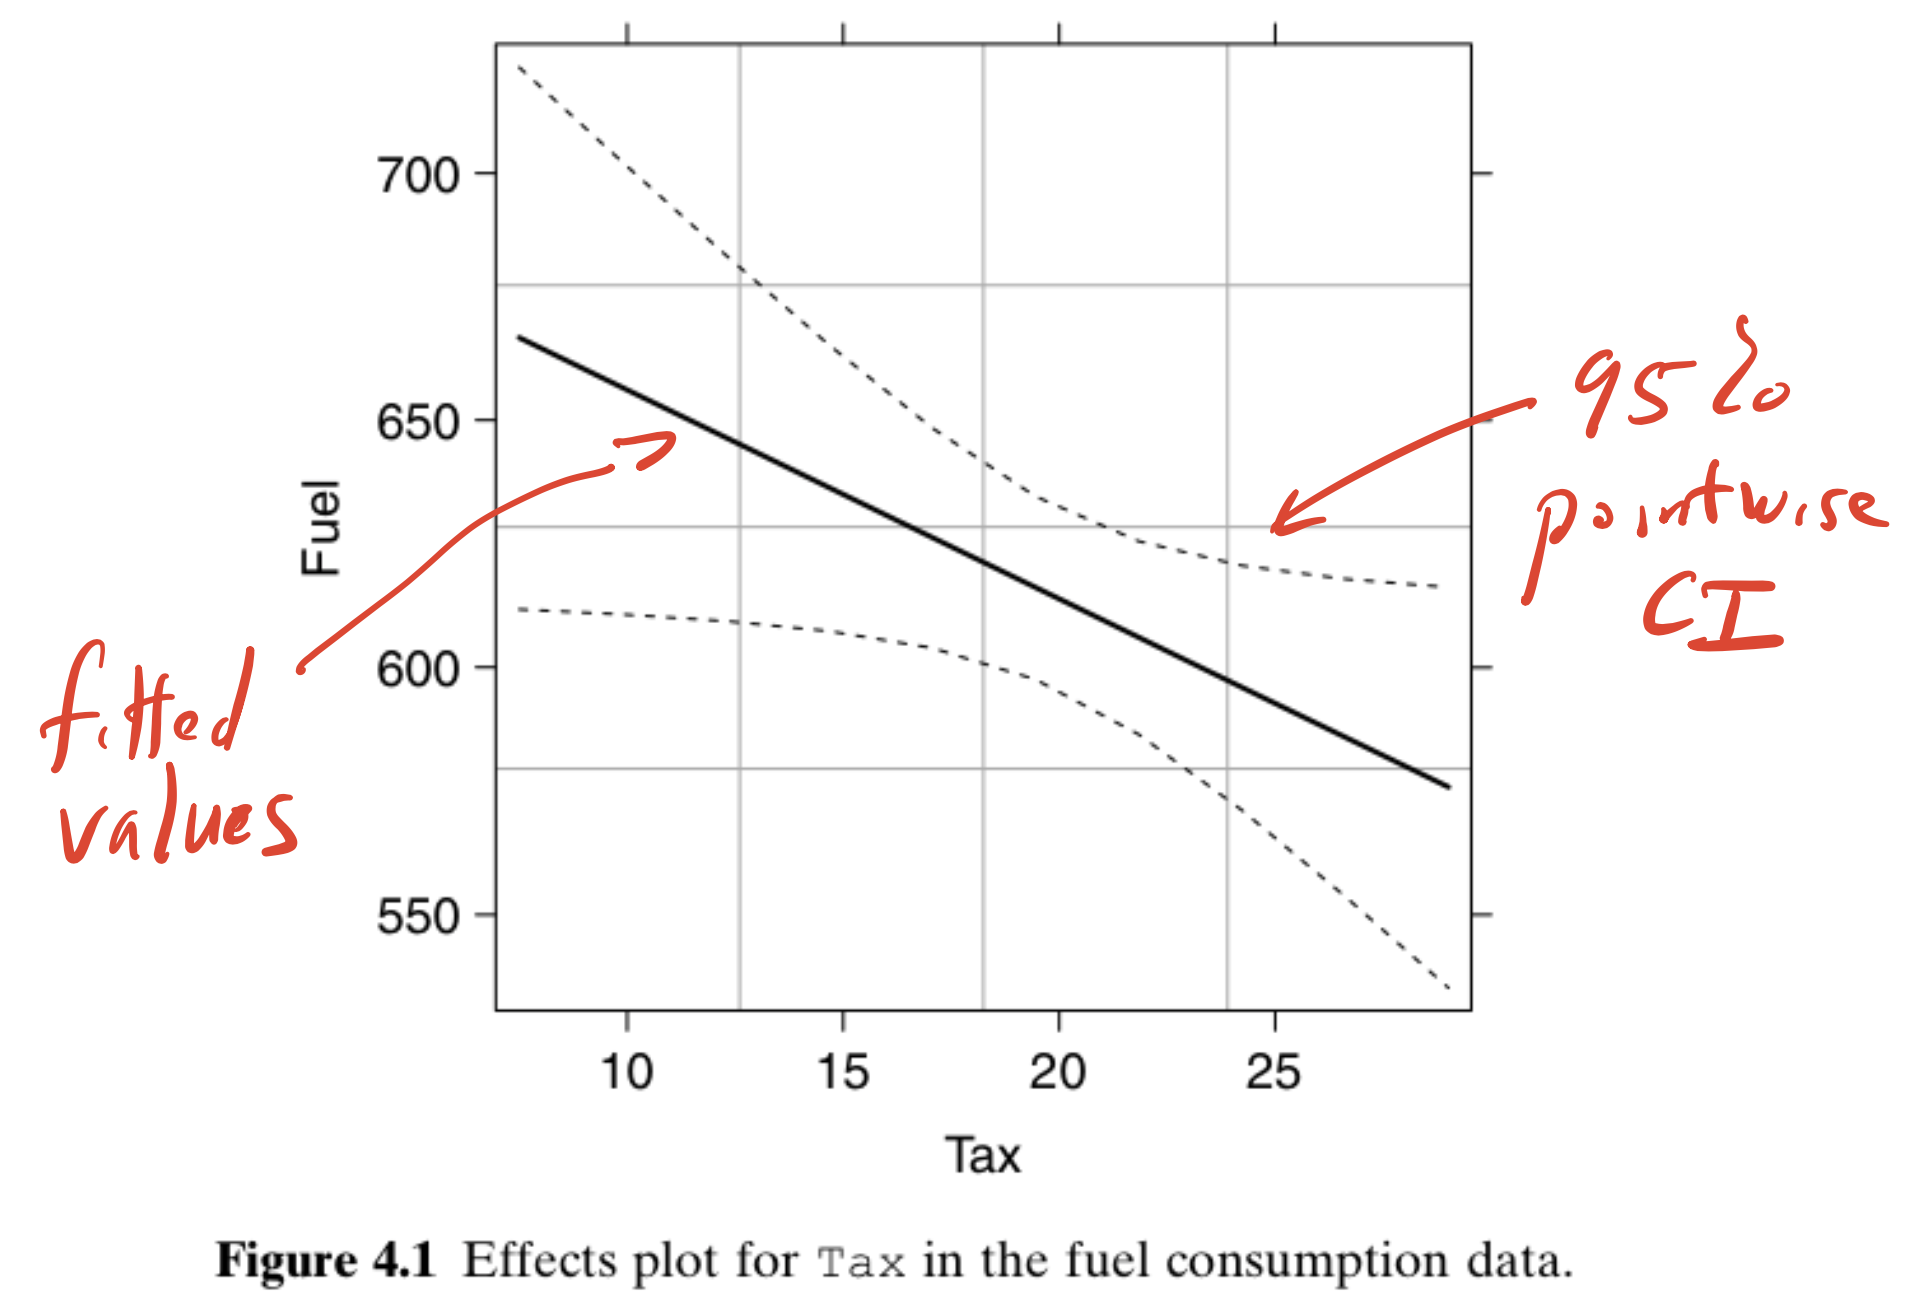
\includegraphics[width=1\textwidth]{fig1.png}
\end{figure}
\[
\Rightarrow \text{Effect of higher } \textcolor{blue}{\text{Tax}} \text{ is lower average } \textcolor{blue}{\text{Fuel}} \text{ consumption}
\]
\[
\textcolor{red}{\text{[not saying anything causal]}}
\]

\section*{Signs of Estimates}

\noindent
Indicates direction of relationship between covariate and response \\
\textcolor{red}{after adjusting for all other covariates in model.} \\
\textcolor{darkgreen}{Caveat: high correlation between covariates can alter both magnitude and sign of an estimated coefficient }\textcolor{blue}{depending on the other covariates in model.}
\begin{figure}[H]
    \centering
    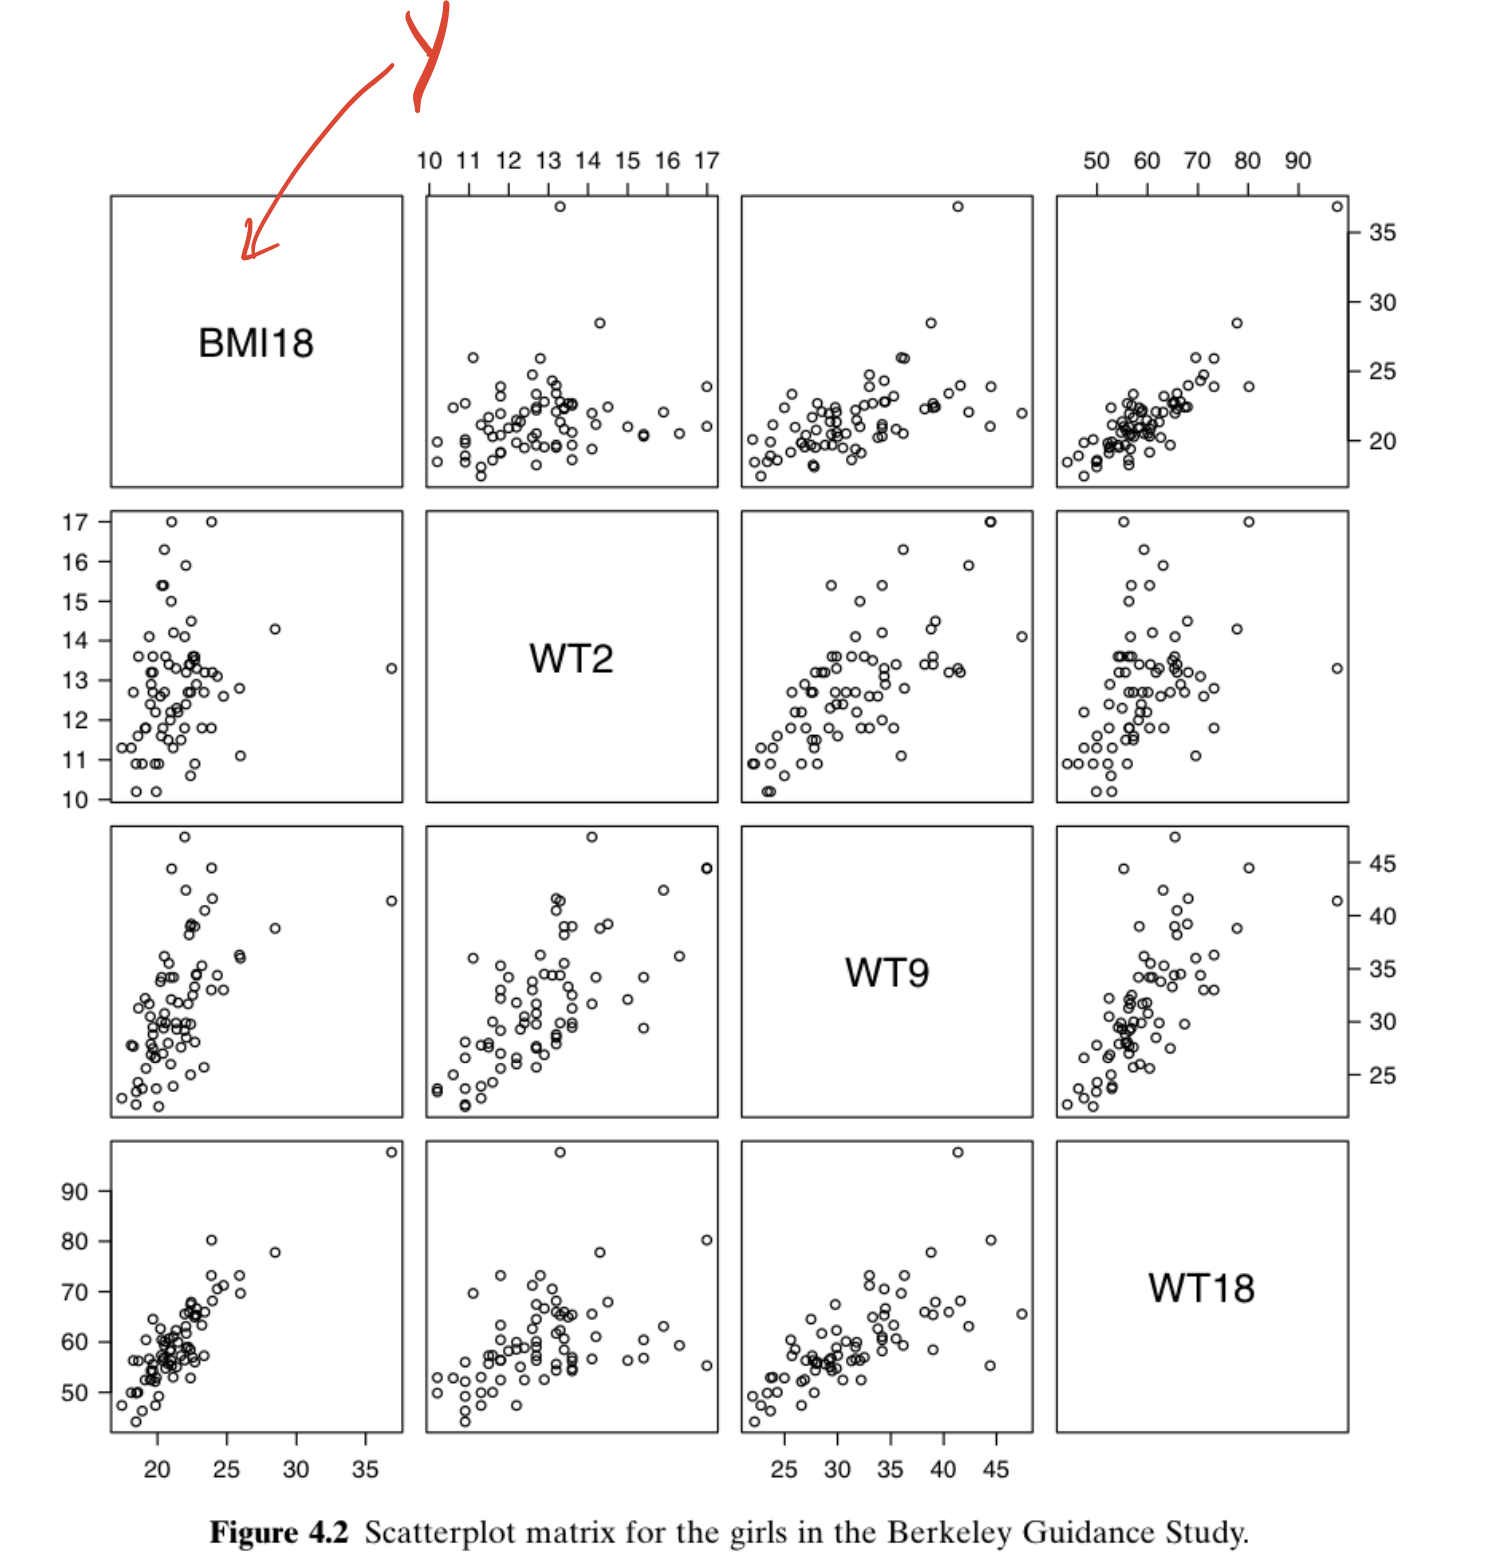
\includegraphics[width=1\textwidth]{fig2.png}
    \textcolor{red}{WT2, WT9, WT18 are covariates}
\end{figure}

\begin{figure}[H]
    \centering
    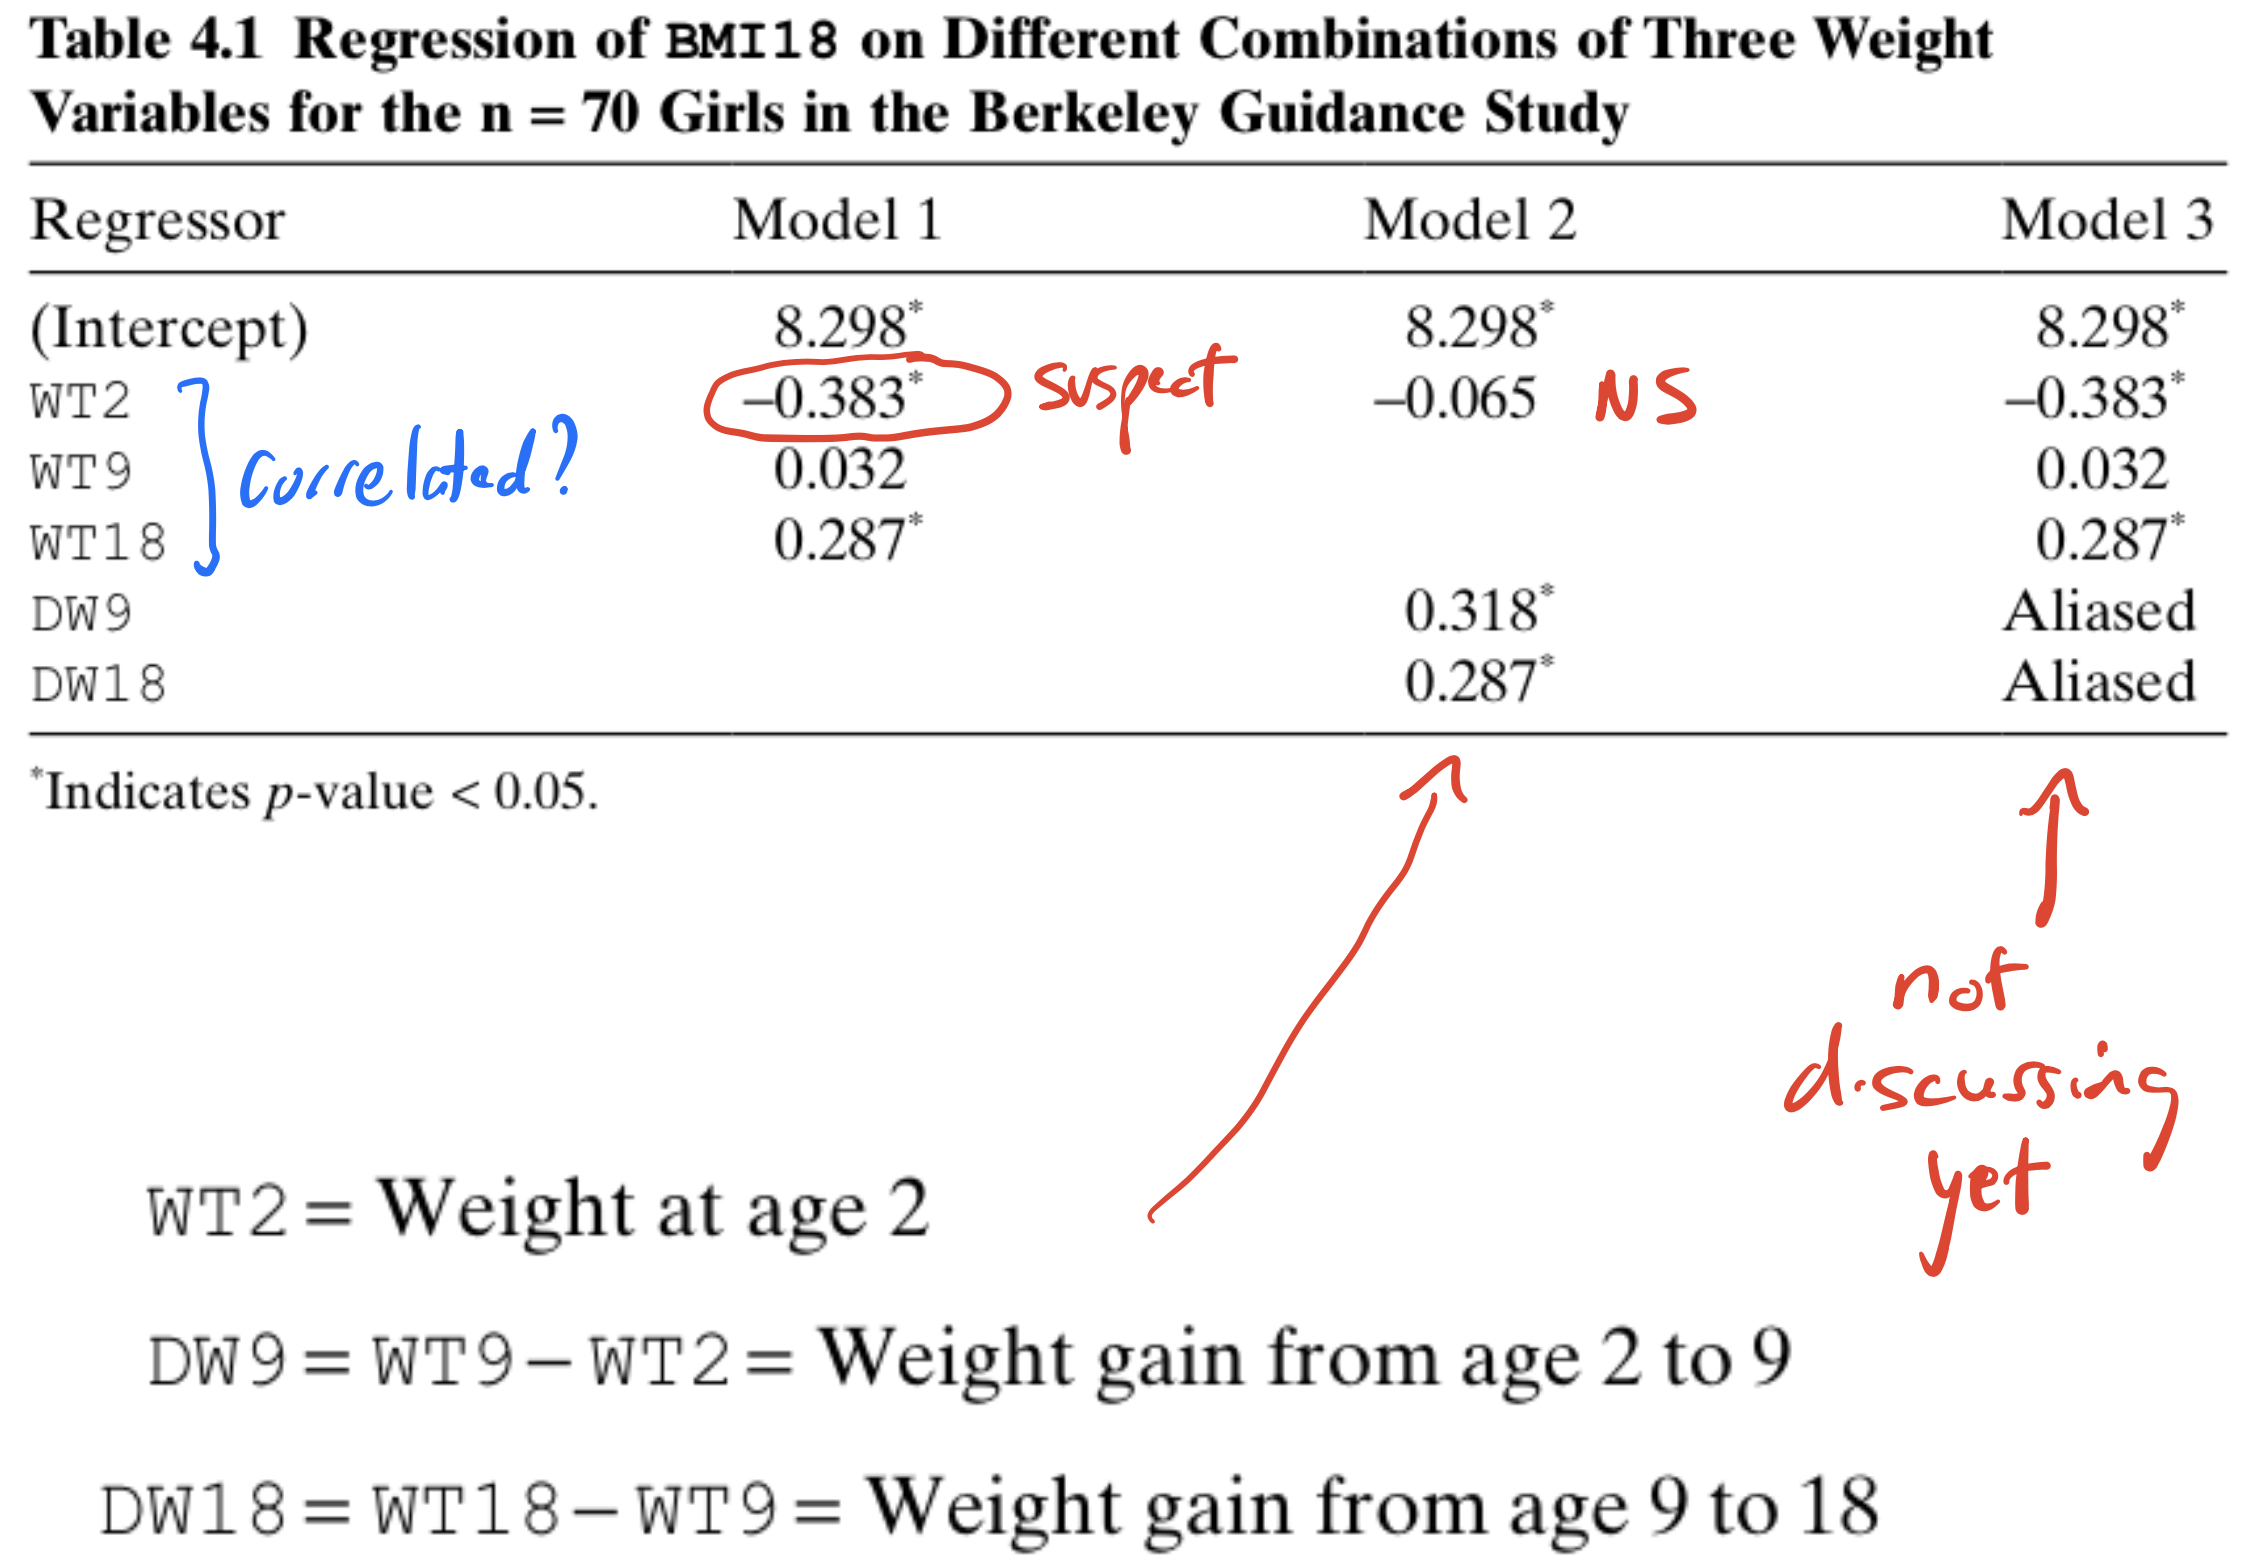
\includegraphics[width=1\textwidth]{fig3.png}
    \textcolor{red}{Redefine covariates}
\end{figure}

\section*{Collinearity}

\noindent
Let $X_{n \times p}$ be data matrix of covariates from sample. \\
If we can find a vector of constants ``$a$'' such that $X_a \approx 0$
\[
\Rightarrow \text{ Covariates are collinear}
\]
if $X_a = 0$
\[
\Rightarrow \text{ over-parameterized model}
\]
\begin{figure}[H]
    \centering
    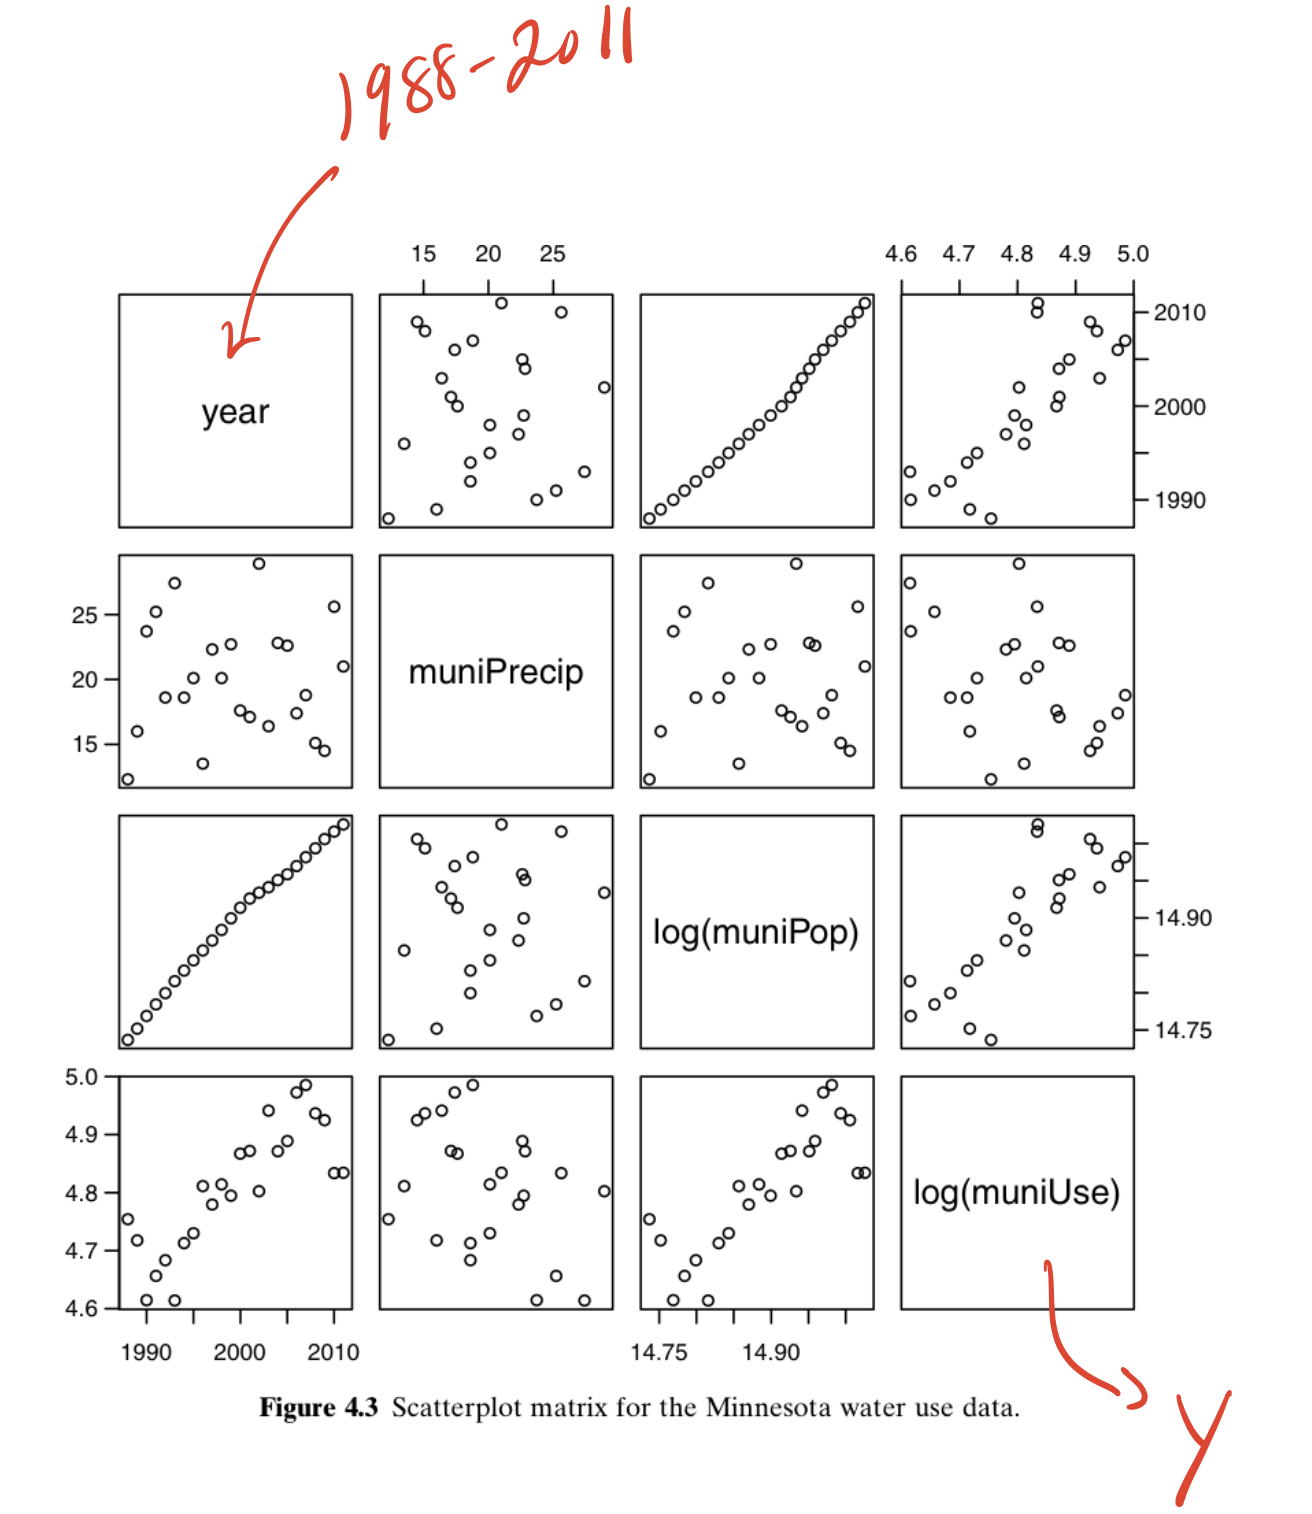
\includegraphics[width=1\textwidth]{fig4.png}
\end{figure}
\begin{figure}[H]
    \centering
    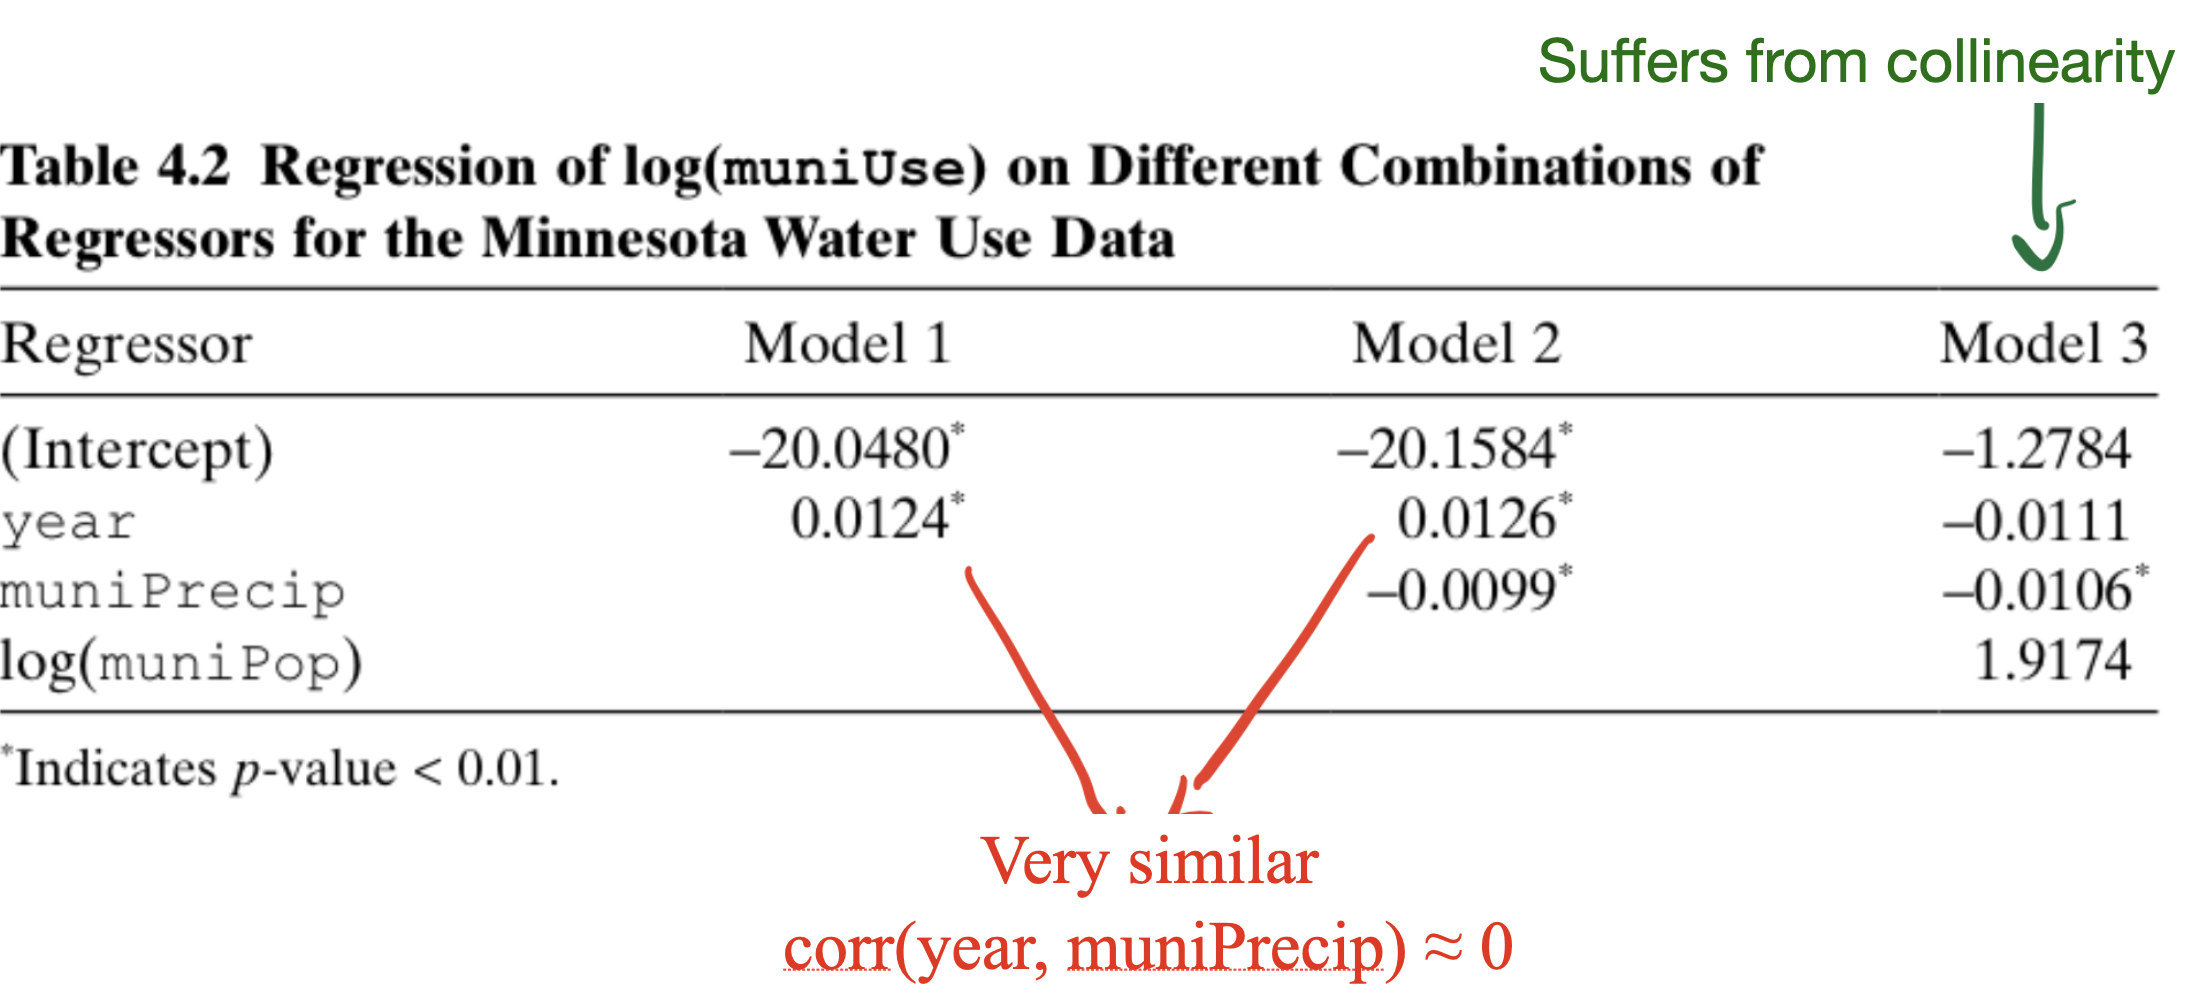
\includegraphics[width=1\textwidth]{fig5.png}
\end{figure}

\section*{Regressors On Logarithmic Scale}

\begin{figure}[H]
    \centering
    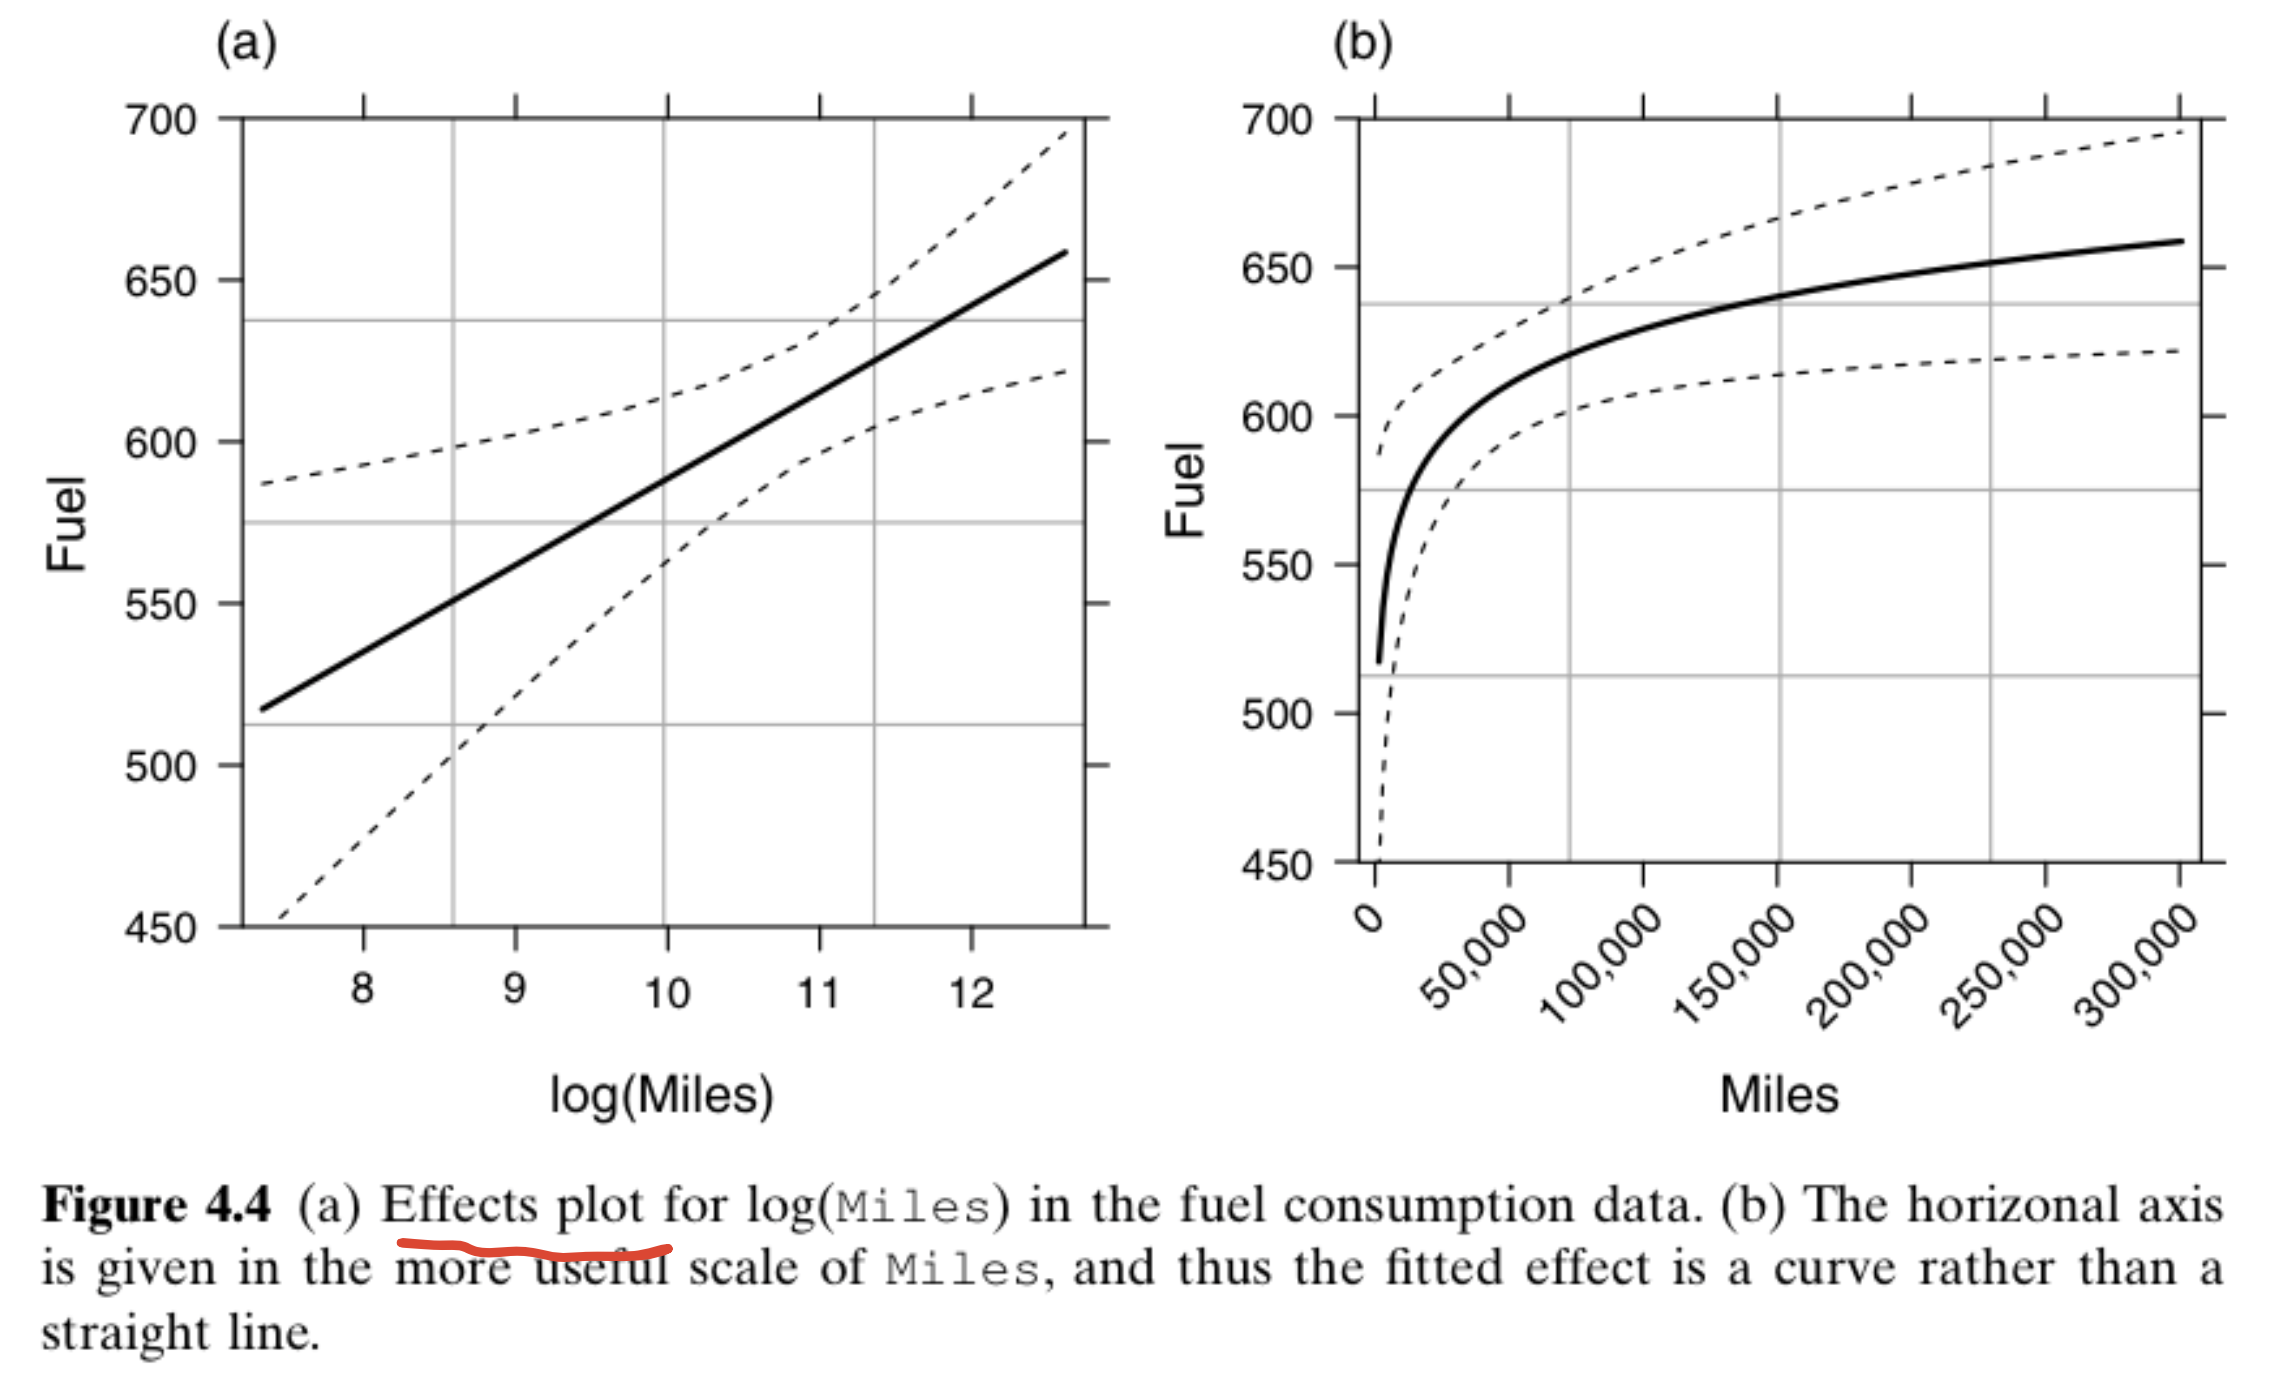
\includegraphics[width=1\textwidth]{fig6.png}
\end{figure}
\noindent
Usual effect of logarithms: \\
\quad fitted effects that change most rapidly when predictor is small

\section*{Response on Logarithmic Scale}

\noindent
Consider model
\[
E(\log(Y) \mid X_j = x_j, \underbrace{X_{(j)} = x_{(j)}}_{\textcolor{red}{\text{predictors excluding }}}) = \beta_0 + \beta_j x_j + \beta'_{(j)} \underbrace{x_{(j)}}_{\textcolor{red}{vector}}
\]
Now approximate LHS by log of expected value:
\[
\log E(Y \mid X_j = x_j, X_{(j)} = x_{(j)}) \approx E \left[ \log(Y) \mid X_j = x_j, X_{(j)} = x_{(j)} \right]
\]
Exponentiate both sides:
\[
E \left[ Y \mid X_j = x_j, X_{(j)} = x_{(j)} \right] \approx \exp \left( E \left[ \log(Y) \mid X_j = x_j, X_{(j)} = x_{(j)} \right] \right)
\]
\[
= \exp \left( \beta_0 + \beta_j x_j + \beta_{(j)}' x_{(j)} \right)
\]
\[
= \exp(\beta_j x_j) \exp \left( \beta_0 + \beta_{(j)}' x_{(j)} \right)
\]
\[
\Rightarrow E \left[ Y \mid X_j = x_j + 1, X_{(j)} = x_{(j)} \right] \approx \exp(\beta_j (x_j + 1)) \exp \left( \beta_0 + \beta_{(j)}' x_{(j)} \right)
\]
\[
= \exp(\beta_j) \exp(\beta_0 + \beta_j x_j + \beta_{(j)}' x_{(j)})
\]
\[
= \exp(\beta_j) \left[ E \left( Y \mid X_j = x_j, X_{(j)} = x_{(j)} \right) \right]
\]
\noindent
$\therefore$ increasing any $x_j$ by 1 will \textcolor{blue}{multiply} the mean of $Y$ by approximately $\exp(\beta_j)$.\\
Can express as a percent change:
\[
100 \times \frac{E \left[ Y \mid X_j = x_j + 1, X_{(j)} = \chi_{(j)} \right] - E \left[ Y \mid X_j = x_j, X_{(j)} = \chi_{(j)} \right]}{E \left[ Y \mid X_j = x_j, X_{(j)} = \chi_{(j)} \right]}
\]
\[
= 100 \left( \exp(\beta_j) - 1 \right)
\]


\subsection*{Example}

\noindent
If $\beta_j = 0.30 \quad \quad \Rightarrow 100 \left( \exp(\beta_j) - 1 \right) = 34\%$ \\
If $\beta_j = -0.20 \quad \Rightarrow 100 \left( \exp(\beta_j) - 1 \right) = -18\% $\\
\textbf{Note:}\\
If both $Y$ and $x_j$ are on the log scale, then $x_j = x_{j+1}$
\[
\Rightarrow \text{multiply } x_j \text{ by } e = 2.718\ldots
\]
(rarely makes sense)

\section*{Dropping Regressors}

\noindent
If regressors are changed, then so are parameters and their interpretations (usually).\\
If $E \left( Y \mid X_1 = x_1, X_2 = x_2 \right)$ is correct $= \beta_0 + \beta_1 x_1 + \beta_2 x_2$\\
What can we say about $E(Y \mid X_1 = x_1)$ ?\\
Can write:
\[
E(Y \mid X_1 = x_1) = E \left[ E(Y \mid X_1 = x_1, X_2) \mid X_1 = x_1 \right] \quad
\]
\[
= \beta_0 + \beta_1' x_1 + \underbrace{\beta_2' E(X_2 \mid X_1 = x_1)}_{\textcolor{red}{\therefore \text{ cannot simply drop } X_2 \text{ regressors from correct model}}}
\]

\section*{Variances when Regressors Dropped}

\[
\text{var}(Y \mid X_1 = x_1)
\]
\[
= E \left[ \text{var}(Y \mid X_1 = x_1, X_2) \mid X_1 = x_1 \right]
\]
\[
+ \text{var} \left[ E(Y \mid X_1 = x_1, X_2) \mid X_1 = x_1 \right]
\]
\[
= \sigma^2 + \beta_2^2 \, \text{var}(X_2 \mid X_1 = x_1) \beta_2
\]

\section*{Sampling From a Normal Population}

\noindent
Suppose
\[
\begin{pmatrix}
X_i \\
Y_i
\end{pmatrix}
\sim \mathcal{N} \left(
\begin{pmatrix}
\mu_X \\
\mu_Y
\end{pmatrix},
\begin{pmatrix}
\sigma_X^2 & \text{cov}(X, Y) \\
\text{cov}(X, Y) & \sigma_Y^2
\end{pmatrix}
\right)
\]
$\therefore$ assume \textcolor{blue}{\text{data pairs}} $\left\{ (x_i, y_i); i = 1, \dots, n \right\}$ are realizations of bivariate normal random variables $X, Y$.\\
Can show
\[
Y_i \mid X_i \sim \mathcal{N} \left( \mu_Y + \rho_{XY} \frac{\sigma_Y}{\sigma_X} (X_i - \mu_X), \sigma_Y^2 (1 - \rho_{XY}^2) \right)
\]
Where
\[
\text{cov}(X, Y) = \rho_{XY} \sigma_X \sigma_Y
\]
Now define
\[
\beta_0 = \mu_Y - \beta_1 \mu_X
\]
\[
\beta_1 = \rho_{XY} \frac{\sigma_Y}{\sigma_X}
\]
\[
\sigma^2 = \sigma_Y^2 (1 - \rho_{XY}^2)
\]
\[
\Rightarrow Y_i \mid X_i \sim \mathcal{N}(\beta_0 + \beta_1 X_i, \sigma^2)
\]
\[
\equiv \text{ SLR with normality assumption added.}
\]
\[
\sigma^2 = \sigma_Y^2 (1 - \rho_{XY}^2) \quad \text{called \textcolor{blue}{residual variance}}
\]
\[
\text{(part of } Y \text{ not explained by } X \text{)}
\]
\textbf{Usual sample estimates under random sampling}
\[
\hat{\mu}_X = \bar{x} \quad \hat{\mu}_Y = \bar{y}
\]
\[
\hat{\sigma}_X^2 = S_X^2 \quad \hat{\sigma}_Y^2 = S_Y^2
\]
\[
\hat{\rho}_{XY} = r_{XY}
\]

\section*{Maximum Likelihood Estimators (MLE)}

\[
Y_i \mid X_i = \mathcal{N}(\beta' X_i, \sigma^2) \quad \text{\textcolor{red}{[more general MLR case]}}
\]
\[
f(Y_i \mid X_i) = \frac{1}{\sqrt{2 \pi \sigma}} \exp \left[ -\frac{(Y_i - \beta' X_i)^2}{2 \sigma^2} \right]
\]
\noindent
from sample of \textcolor{red}{(independent)} data $\{(x_i, y_i); i = 1, \dots, n\}$
\[
L(\beta, \sigma^2 \mid y_1, \dots, y_n) = \prod_{i=1}^{n} f(y_i \mid x_i; \beta, \sigma^2)
\]
\[
= \left( \frac{1}{\sqrt{2 \pi \sigma^2}} \right)^n \exp \left[ -\frac{1}{\sigma^2} \sum_{i=1}^{n} (y_i - \beta' x_i)^2 \right]
\]
\[
\log L(\beta, \sigma^2 \mid y_1, \dots, y_n) = -\frac{n}{2} (\log 2 \pi) - \frac{n}{2} \log(\sigma^2) - \frac{1}{2 \sigma^2} \sum_{i=1}^{n} (y_i - \beta' x_i)^2
\]
What this shows is that
\[
\hat{\beta}^{\text{MLE}} = \hat{\beta}^{\text{OLS}}
\]
Then
\[
\hat{\sigma}_{\text{MLE}}^2 = \text{RSS} / n \quad \left[ \text{not } \frac{\text{RSS}}{(n - (p + 1))} \right]
\]
\textcolor{blue}{MLE theory has some attractive theoretical properties}\\
\textcolor{red}{e.g., UMVUE, normality or asymptotic normality}

\newpage

\section*{MLR and $R^2$}
\begin{figure}[H]
    \centering
    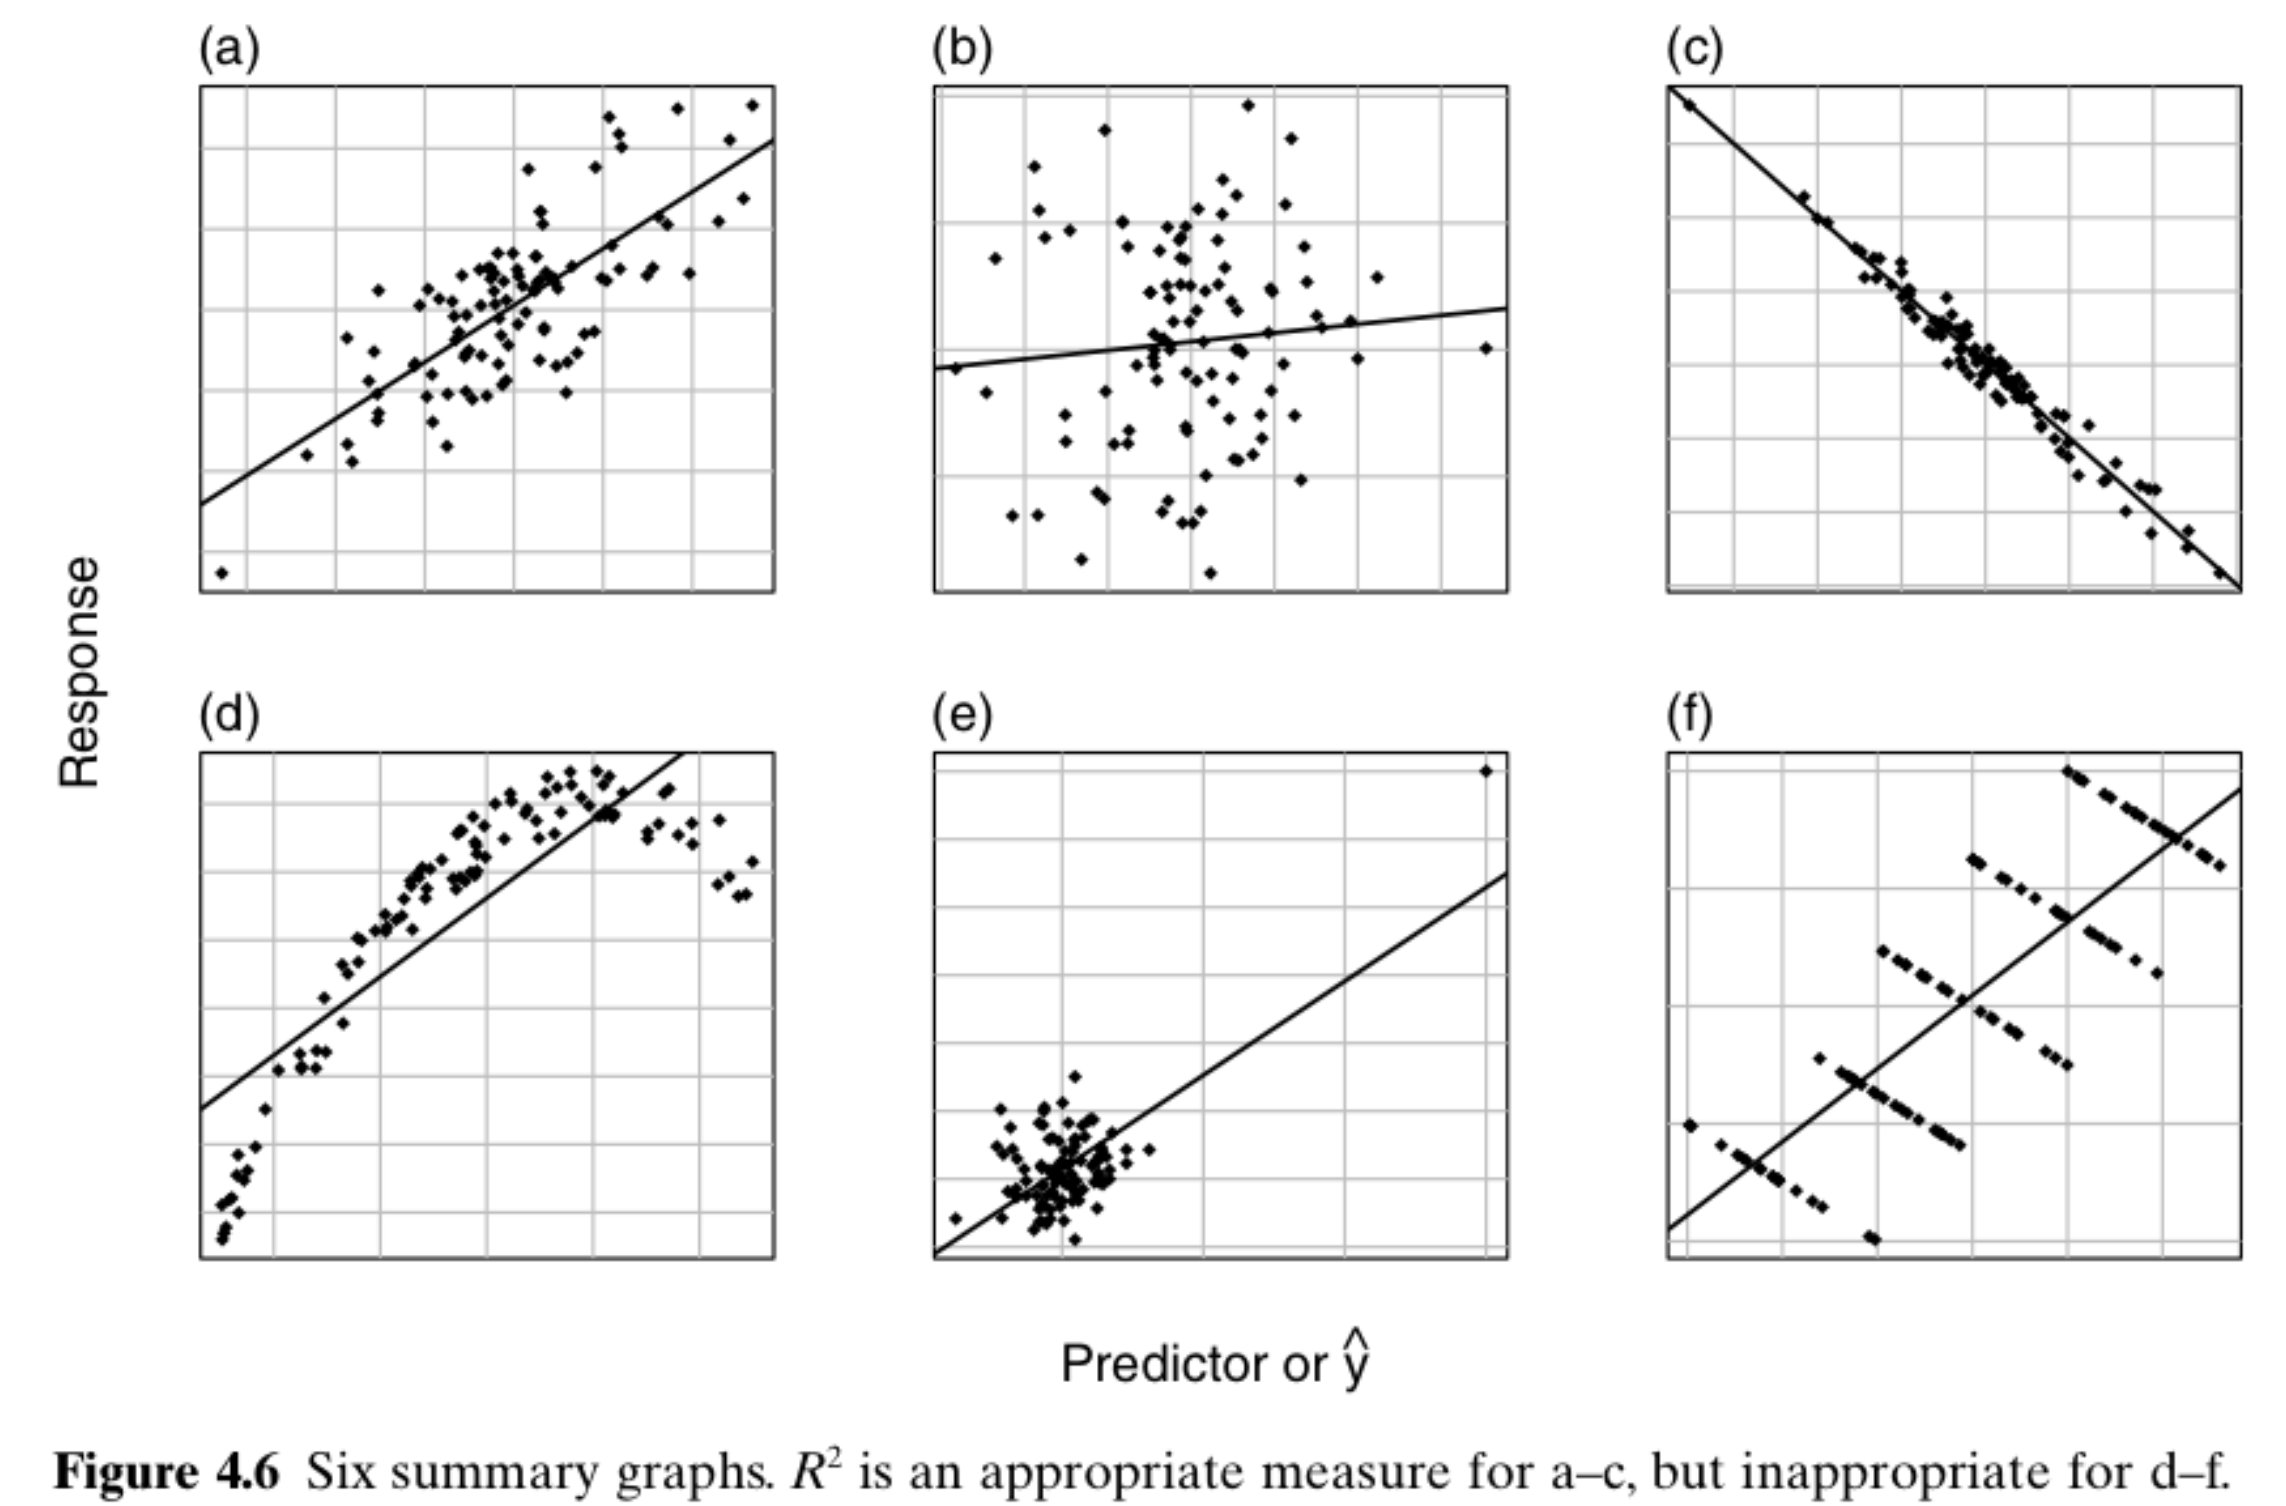
\includegraphics[width=1\textwidth]{fig7.png}
\end{figure}
\[
R^2 \equiv \text{corr}(Y, \hat{Y})
\quad \text{\textcolor{red}{[one can show this]}}
\]

\section*{Regression through Origin and $R^2$}

\noindent
\[
\text{prop of variability explained} = 1 - \frac{\text{RSS}}{\sum_{i=1}^{n} y_i^2}
\]
\textcolor{red}{Not invariant under location change.}\\
\textcolor{red}{(e.g., going from $^\circ$F to $^\circ$C, $R^2$ changes)}\\
\text{\textcolor{blue}{$\therefore R^2$ use here not recommended.}}



\end{document}